\documentclass[1p]{elsarticle_modified}
%\bibliographystyle{elsarticle-num}

%\usepackage[colorlinks]{hyperref}
%\usepackage{abbrmath_seonhwa} %\Abb, \Ascr, \Acal ,\Abf, \Afrak
\usepackage{amsfonts}
\usepackage{amssymb}
\usepackage{amsmath}
\usepackage{amsthm}
\usepackage{scalefnt}
\usepackage{amsbsy}
\usepackage{kotex}
\usepackage{caption}
\usepackage{subfig}
\usepackage{color}
\usepackage{graphicx}
\usepackage{xcolor} %% white, black, red, green, blue, cyan, magenta, yellow
\usepackage{float}
\usepackage{setspace}
\usepackage{hyperref}

\usepackage{tikz}
\usetikzlibrary{arrows}

\usepackage{multirow}
\usepackage{array} % fixed length table
\usepackage{hhline}

%%%%%%%%%%%%%%%%%%%%%
\makeatletter
\renewcommand*\env@matrix[1][\arraystretch]{%
	\edef\arraystretch{#1}%
	\hskip -\arraycolsep
	\let\@ifnextchar\new@ifnextchar
	\array{*\c@MaxMatrixCols c}}
\makeatother %https://tex.stackexchange.com/questions/14071/how-can-i-increase-the-line-spacing-in-a-matrix
%%%%%%%%%%%%%%%

\usepackage[normalem]{ulem}

\newcommand{\msout}[1]{\ifmmode\text{\sout{\ensuremath{#1}}}\else\sout{#1}\fi}
%SOURCE: \msout is \stkout macro in https://tex.stackexchange.com/questions/20609/strikeout-in-math-mode

\newcommand{\cancel}[1]{
	\ifmmode
	{\color{red}\msout{#1}}
	\else
	{\color{red}\sout{#1}}
	\fi
}

\newcommand{\add}[1]{
	{\color{blue}\uwave{#1}}
}

\newcommand{\replace}[2]{
	\ifmmode
	{\color{red}\msout{#1}}{\color{blue}\uwave{#2}}
	\else
	{\color{red}\sout{#1}}{\color{blue}\uwave{#2}}
	\fi
}

\newcommand{\Sol}{\mathcal{S}} %segment
\newcommand{\D}{D} %diagram
\newcommand{\A}{\mathcal{A}} %arc


%%%%%%%%%%%%%%%%%%%%%%%%%%%%%5 test

\def\sl{\operatorname{\textup{SL}}(2,\Cbb)}
\def\psl{\operatorname{\textup{PSL}}(2,\Cbb)}
\def\quan{\mkern 1mu \triangleright \mkern 1mu}

\theoremstyle{definition}
\newtheorem{thm}{Theorem}[section]
\newtheorem{prop}[thm]{Proposition}
\newtheorem{lem}[thm]{Lemma}
\newtheorem{ques}[thm]{Question}
\newtheorem{cor}[thm]{Corollary}
\newtheorem{defn}[thm]{Definition}
\newtheorem{exam}[thm]{Example}
\newtheorem{rmk}[thm]{Remark}
\newtheorem{alg}[thm]{Algorithm}

\newcommand{\I}{\sqrt{-1}}
\begin{document}

%\begin{frontmatter}
%
%\title{Boundary parabolic representations of knots up to 8 crossings}
%
%%% Group authors per affiliation:
%\author{Yunhi Cho} 
%\address{Department of Mathematics, University of Seoul, Seoul, Korea}
%\ead{yhcho@uos.ac.kr}
%
%
%\author{Seonhwa Kim} %\fnref{s_kim}}
%\address{Center for Geometry and Physics, Institute for Basic Science, Pohang, 37673, Korea}
%\ead{ryeona17@ibs.re.kr}
%
%\author{Hyuk Kim}
%\address{Department of Mathematical Sciences, Seoul National University, Seoul 08826, Korea}
%\ead{hyukkim@snu.ac.kr}
%
%\author{Seokbeom Yoon}
%\address{Department of Mathematical Sciences, Seoul National University, Seoul, 08826,  Korea}
%\ead{sbyoon15@snu.ac.kr}
%
%\begin{abstract}
%We find all boundary parabolic representation of knots up to 8 crossings.
%
%\end{abstract}
%\begin{keyword}
%    \MSC[2010] 57M25 
%\end{keyword}
%
%\end{frontmatter}

%\linenumbers
%\tableofcontents
%
\newcommand\colored[1]{\textcolor{white}{\rule[-0.35ex]{0.8em}{1.4ex}}\kern-0.8em\color{red} #1}%
%\newcommand\colored[1]{\textcolor{white}{ #1}\kern-2.17ex	\textcolor{white}{ #1}\kern-1.81ex	\textcolor{white}{ #1}\kern-2.15ex\color{red}#1	}

{\Large $\underline{12n_{0599}~(K12n_{0599})}$}

\setlength{\tabcolsep}{10pt}
\renewcommand{\arraystretch}{1.6}
\vspace{1cm}\begin{tabular}{m{100pt}>{\centering\arraybackslash}m{274pt}}
\multirow{5}{120pt}{
	\centering
	\includegraphics[width=112pt]{../../../GIT/diagram.site/Diagrams/png/2688_12n_0599.png}\\
\ \ \ A knot diagram\footnotemark}&
\allowdisplaybreaks
\textbf{Linearized knot diagam} \\
\cline{2-2}
 &
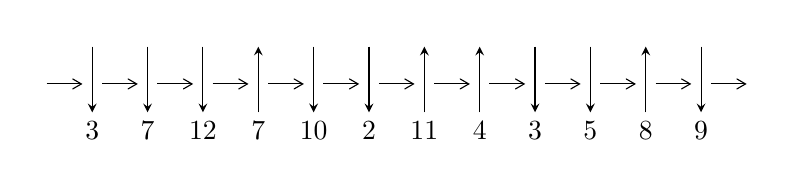
\begin{tikzpicture}[x=20pt, y=17pt]
	% nodes
	\node (C0) at (0, 0) {};
	\node (C1) at (1, 0) {};
	\node (C1U) at (1, +1) {};
	\node (C1D) at (1, -1) {3};

	\node (C2) at (2, 0) {};
	\node (C2U) at (2, +1) {};
	\node (C2D) at (2, -1) {7};

	\node (C3) at (3, 0) {};
	\node (C3U) at (3, +1) {};
	\node (C3D) at (3, -1) {12};

	\node (C4) at (4, 0) {};
	\node (C4U) at (4, +1) {};
	\node (C4D) at (4, -1) {7};

	\node (C5) at (5, 0) {};
	\node (C5U) at (5, +1) {};
	\node (C5D) at (5, -1) {10};

	\node (C6) at (6, 0) {};
	\node (C6U) at (6, +1) {};
	\node (C6D) at (6, -1) {2};

	\node (C7) at (7, 0) {};
	\node (C7U) at (7, +1) {};
	\node (C7D) at (7, -1) {11};

	\node (C8) at (8, 0) {};
	\node (C8U) at (8, +1) {};
	\node (C8D) at (8, -1) {4};

	\node (C9) at (9, 0) {};
	\node (C9U) at (9, +1) {};
	\node (C9D) at (9, -1) {3};

	\node (C10) at (10, 0) {};
	\node (C10U) at (10, +1) {};
	\node (C10D) at (10, -1) {5};

	\node (C11) at (11, 0) {};
	\node (C11U) at (11, +1) {};
	\node (C11D) at (11, -1) {8};

	\node (C12) at (12, 0) {};
	\node (C12U) at (12, +1) {};
	\node (C12D) at (12, -1) {9};
	\node (C13) at (13, 0) {};

	% arrows
	\draw[->,>={angle 60}]
	(C0) edge (C1) (C1) edge (C2) (C2) edge (C3) (C3) edge (C4) (C4) edge (C5) (C5) edge (C6) (C6) edge (C7) (C7) edge (C8) (C8) edge (C9) (C9) edge (C10) (C10) edge (C11) (C11) edge (C12) (C12) edge (C13) ;	\draw[->,>=stealth]
	(C1U) edge (C1D) (C2U) edge (C2D) (C3U) edge (C3D) (C4D) edge (C4U) (C5U) edge (C5D) (C6U) edge (C6D) (C7D) edge (C7U) (C8D) edge (C8U) (C9U) edge (C9D) (C10U) edge (C10D) (C11D) edge (C11U) (C12U) edge (C12D) ;
	\end{tikzpicture} \\
\hhline{~~} \\& 
\textbf{Solving Sequence} \\ \cline{2-2} 
 &
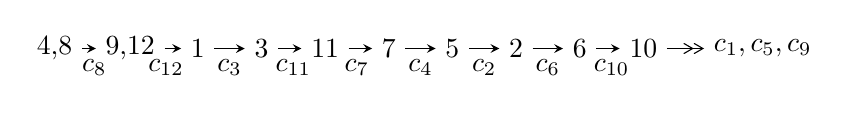
\begin{tikzpicture}[x=23pt, y=7pt]
	% node
	\node (A0) at (-1/8, 0) {4,8};
	\node (A1) at (17/16, 0) {9,12};
	\node (A2) at (17/8, 0) {1};
	\node (A3) at (25/8, 0) {3};
	\node (A4) at (33/8, 0) {11};
	\node (A5) at (41/8, 0) {7};
	\node (A6) at (49/8, 0) {5};
	\node (A7) at (57/8, 0) {2};
	\node (A8) at (65/8, 0) {6};
	\node (A9) at (73/8, 0) {10};
	\node (C1) at (1/2, -1) {$c_{8}$};
	\node (C2) at (13/8, -1) {$c_{12}$};
	\node (C3) at (21/8, -1) {$c_{3}$};
	\node (C4) at (29/8, -1) {$c_{11}$};
	\node (C5) at (37/8, -1) {$c_{7}$};
	\node (C6) at (45/8, -1) {$c_{4}$};
	\node (C7) at (53/8, -1) {$c_{2}$};
	\node (C8) at (61/8, -1) {$c_{6}$};
	\node (C9) at (69/8, -1) {$c_{10}$};
	\node (A10) at (11, 0) {$c_{1},c_{5},c_{9}$};

	% edge
	\draw[->,>=stealth]	
	(A0) edge (A1) (A1) edge (A2) (A2) edge (A3) (A3) edge (A4) (A4) edge (A5) (A5) edge (A6) (A6) edge (A7) (A7) edge (A8) (A8) edge (A9) ;
	\draw[->>,>={angle 60}]	
	(A9) edge (A10);
\end{tikzpicture} \\ 

\end{tabular} \\

\footnotetext{
The image of knot diagram is generated by the software ``\textbf{Draw programme}" developed by Andrew Bartholomew(\url{http://www.layer8.co.uk/maths/draw/index.htm\#Running-draw}), where we modified some parts for our purpose(\url{https://github.com/CATsTAILs/LinksPainter}).
}\phantom \\ \newline 
\centering \textbf{Ideals for irreducible components\footnotemark of $X_{\text{par}}$} 
 
\begin{align*}
I^u_{1}&=\langle 
2.08585\times10^{97} u^{41}+7.14533\times10^{97} u^{40}+\cdots+2.87929\times10^{99} b+1.73918\times10^{99},\\
\phantom{I^u_{1}}&\phantom{= \langle  }5.30575\times10^{95} u^{41}+1.71743\times10^{97} u^{40}+\cdots+1.43964\times10^{99} a-9.16089\times10^{98},\;u^{42}+3 u^{41}+\cdots+64 u+32\rangle \\
I^u_{2}&=\langle 
4075773832297 u^{14}-2172521972436 u^{13}+\cdots+11315912876891 b-9436584195071,\\
\phantom{I^u_{2}}&\phantom{= \langle  }12204692706877 u^{14}-2379455879777 u^{13}+\cdots+11315912876891 a-25876335477767,\\
\phantom{I^u_{2}}&\phantom{= \langle  }u^{15}-5 u^{13}-10 u^{12}-23 u^{11}-49 u^{10}-54 u^9-6 u^8-42 u^7-27 u^6-4 u^5+12 u^4+20 u^3+11 u^2+2 u+1\rangle \\
\\
\end{align*}
\raggedright * 2 irreducible components of $\dim_{\mathbb{C}}=0$, with total 57 representations.\\
\footnotetext{All coefficients of polynomials are rational numbers. But the coefficients are sometimes approximated in decimal forms when there is not enough margin.}
\newpage
\renewcommand{\arraystretch}{1}
\centering \section*{I. $I^u_{1}= \langle 2.09\times10^{97} u^{41}+7.15\times10^{97} u^{40}+\cdots+2.88\times10^{99} b+1.74\times10^{99},\;5.31\times10^{95} u^{41}+1.72\times10^{97} u^{40}+\cdots+1.44\times10^{99} a-9.16\times10^{98},\;u^{42}+3 u^{41}+\cdots+64 u+32 \rangle$}
\flushleft \textbf{(i) Arc colorings}\\
\begin{tabular}{m{7pt} m{180pt} m{7pt} m{180pt} }
\flushright $a_{4}=$&$\begin{pmatrix}0\\u\end{pmatrix}$ \\
\flushright $a_{8}=$&$\begin{pmatrix}1\\0\end{pmatrix}$ \\
\flushright $a_{9}=$&$\begin{pmatrix}1\\- u^2\end{pmatrix}$ \\
\flushright $a_{12}=$&$\begin{pmatrix}-0.000368546 u^{41}-0.0119295 u^{40}+\cdots+10.1776 u+0.636330\\-0.00724434 u^{41}-0.0248163 u^{40}+\cdots+5.49278 u-0.604030\end{pmatrix}$ \\
\flushright $a_{1}=$&$\begin{pmatrix}0.00215244 u^{41}+0.000734500 u^{40}+\cdots+3.98031 u+0.893995\\-0.00639184 u^{41}-0.0228879 u^{40}+\cdots+5.89992 u-0.440795\end{pmatrix}$ \\
\flushright $a_{3}=$&$\begin{pmatrix}0.00520650 u^{41}+0.0133533 u^{40}+\cdots+5.05203 u+1.97585\\0.0108948 u^{41}+0.0265127 u^{40}+\cdots+3.13035 u+0.813921\end{pmatrix}$ \\
\flushright $a_{11}=$&$\begin{pmatrix}0.00687579 u^{41}+0.0128868 u^{40}+\cdots+4.68483 u+1.24036\\-0.00724434 u^{41}-0.0248163 u^{40}+\cdots+5.49278 u-0.604030\end{pmatrix}$ \\
\flushright $a_{7}=$&$\begin{pmatrix}-0.0284111 u^{41}-0.0802538 u^{40}+\cdots+5.73043 u+0.660082\\0.00297602 u^{41}+0.0148436 u^{40}+\cdots-6.80600 u+0.842424\end{pmatrix}$ \\
\flushright $a_{5}=$&$\begin{pmatrix}0.00358475 u^{41}+0.0184991 u^{40}+\cdots-1.07592 u+1.21549\\0.0129804 u^{41}+0.0337132 u^{40}+\cdots+2.17091 u+1.68243\end{pmatrix}$ \\
\flushright $a_{2}=$&$\begin{pmatrix}0.0241930 u^{41}+0.0654847 u^{40}+\cdots+11.3542 u+2.32053\\-0.00534000 u^{41}-0.0268669 u^{40}+\cdots+8.37009 u-1.59602\end{pmatrix}$ \\
\flushright $a_{6}=$&$\begin{pmatrix}-0.0377424 u^{41}-0.120931 u^{40}+\cdots+1.19694 u-1.53872\\-0.0110412 u^{41}-0.0237259 u^{40}+\cdots-0.776747 u-1.63777\end{pmatrix}$ \\
\flushright $a_{10}=$&$\begin{pmatrix}0.0131333 u^{41}+0.0397783 u^{40}+\cdots+8.14332 u+1.94601\\-0.00917113 u^{41}-0.0293322 u^{40}+\cdots+2.00016 u-1.60632\end{pmatrix}$\\&\end{tabular}
\flushleft \textbf{(ii) Obstruction class $= -1$}\\~\\
\flushleft \textbf{(iii) Cusp Shapes $= -0.0471714 u^{41}-0.112106 u^{40}+\cdots-28.6268 u-3.86134$}\\~\\
\newpage\renewcommand{\arraystretch}{1}
\flushleft \textbf{(iv) u-Polynomials at the component}\newline \\
\begin{tabular}{m{50pt}|m{274pt}}
Crossings & \hspace{64pt}u-Polynomials at each crossing \\
\hline $$\begin{aligned}c_{1}\end{aligned}$$&$\begin{aligned}
&u^{42}+64 u^{41}+\cdots-161335 u+1849
\end{aligned}$\\
\hline $$\begin{aligned}c_{2},c_{6}\end{aligned}$$&$\begin{aligned}
&u^{42}+2 u^{41}+\cdots-601 u+43
\end{aligned}$\\
\hline $$\begin{aligned}c_{3}\end{aligned}$$&$\begin{aligned}
&u^{42}-6 u^{41}+\cdots+16 u-1
\end{aligned}$\\
\hline $$\begin{aligned}c_{4}\end{aligned}$$&$\begin{aligned}
&u^{42}+12 u^{41}+\cdots+3596 u+676
\end{aligned}$\\
\hline $$\begin{aligned}c_{5},c_{10}\end{aligned}$$&$\begin{aligned}
&u^{42}- u^{41}+\cdots-190 u-43
\end{aligned}$\\
\hline $$\begin{aligned}c_{7},c_{11}\end{aligned}$$&$\begin{aligned}
&u^{42}-3 u^{41}+\cdots-11 u-1
\end{aligned}$\\
\hline $$\begin{aligned}c_{8}\end{aligned}$$&$\begin{aligned}
&u^{42}-3 u^{41}+\cdots-64 u+32
\end{aligned}$\\
\hline $$\begin{aligned}c_{9}\end{aligned}$$&$\begin{aligned}
&u^{42}- u^{41}+\cdots-2006840 u+356879
\end{aligned}$\\
\hline $$\begin{aligned}c_{12}\end{aligned}$$&$\begin{aligned}
&u^{42}-29 u^{40}+\cdots-342 u-76
\end{aligned}$\\
\hline
\end{tabular}\\~\\
\newpage\renewcommand{\arraystretch}{1}
\flushleft \textbf{(v) Riley Polynomials at the component}\newline \\
\begin{tabular}{m{50pt}|m{274pt}}
Crossings & \hspace{64pt}Riley Polynomials at each crossing \\
\hline $$\begin{aligned}c_{1}\end{aligned}$$&$\begin{aligned}
&y^{42}-192 y^{41}+\cdots-7743629545 y+3418801
\end{aligned}$\\
\hline $$\begin{aligned}c_{2},c_{6}\end{aligned}$$&$\begin{aligned}
&y^{42}-64 y^{41}+\cdots+161335 y+1849
\end{aligned}$\\
\hline $$\begin{aligned}c_{3}\end{aligned}$$&$\begin{aligned}
&y^{42}+6 y^{41}+\cdots-180 y+1
\end{aligned}$\\
\hline $$\begin{aligned}c_{4}\end{aligned}$$&$\begin{aligned}
&y^{42}+2 y^{41}+\cdots-1564952 y+456976
\end{aligned}$\\
\hline $$\begin{aligned}c_{5},c_{10}\end{aligned}$$&$\begin{aligned}
&y^{42}+3 y^{41}+\cdots-31284 y+1849
\end{aligned}$\\
\hline $$\begin{aligned}c_{7},c_{11}\end{aligned}$$&$\begin{aligned}
&y^{42}-37 y^{41}+\cdots-245 y+1
\end{aligned}$\\
\hline $$\begin{aligned}c_{8}\end{aligned}$$&$\begin{aligned}
&y^{42}+y^{41}+\cdots-27136 y+1024
\end{aligned}$\\
\hline $$\begin{aligned}c_{9}\end{aligned}$$&$\begin{aligned}
&y^{42}-109 y^{41}+\cdots-1736409911214 y+127362620641
\end{aligned}$\\
\hline $$\begin{aligned}c_{12}\end{aligned}$$&$\begin{aligned}
&y^{42}-58 y^{41}+\cdots+99636 y+5776
\end{aligned}$\\
\hline
\end{tabular}\\~\\
\newpage\flushleft \textbf{(vi) Complex Volumes and Cusp Shapes}
$$\begin{array}{c|c|c}  
\text{Solutions to }I^u_{1}& \I (\text{vol} + \sqrt{-1}CS) & \text{Cusp shape}\\
 \hline 
\begin{aligned}
u &= \phantom{-}0.648045 + 0.762828 I \\
a &= -0.199463 - 1.026950 I \\
b &= \phantom{-}0.000607 - 0.888637 I\end{aligned}
 & -2.26225 + 2.79311 I & -8.37862 - 3.97835 I \\ \hline\begin{aligned}
u &= \phantom{-}0.648045 - 0.762828 I \\
a &= -0.199463 + 1.026950 I \\
b &= \phantom{-}0.000607 + 0.888637 I\end{aligned}
 & -2.26225 - 2.79311 I & -8.37862 + 3.97835 I \\ \hline\begin{aligned}
u &= \phantom{-}0.462736 + 0.870276 I \\
a &= \phantom{-}1.082390 + 0.631958 I \\
b &= \phantom{-}1.380710 - 0.068283 I\end{aligned}
 & \phantom{-}7.99084 - 2.22911 I & \phantom{-}4.00956 + 3.14309 I \\ \hline\begin{aligned}
u &= \phantom{-}0.462736 - 0.870276 I \\
a &= \phantom{-}1.082390 - 0.631958 I \\
b &= \phantom{-}1.380710 + 0.068283 I\end{aligned}
 & \phantom{-}7.99084 + 2.22911 I & \phantom{-}4.00956 - 3.14309 I \\ \hline\begin{aligned}
u &= -0.371673 + 0.796152 I \\
a &= \phantom{-}0.020113 + 0.557804 I \\
b &= -0.222389 + 0.704830 I\end{aligned}
 & -0.17172 - 1.89179 I & -2.28677 + 1.75619 I \\ \hline\begin{aligned}
u &= -0.371673 - 0.796152 I \\
a &= \phantom{-}0.020113 - 0.557804 I \\
b &= -0.222389 - 0.704830 I\end{aligned}
 & -0.17172 + 1.89179 I & -2.28677 - 1.75619 I \\ \hline\begin{aligned}
u &= -0.314772 + 0.773309 I \\
a &= -0.38000 + 1.41391 I \\
b &= \phantom{-}1.093270 + 0.667135 I\end{aligned}
 & -10.09930 - 2.74341 I & -5.66707 + 2.17488 I \\ \hline\begin{aligned}
u &= -0.314772 - 0.773309 I \\
a &= -0.38000 - 1.41391 I \\
b &= \phantom{-}1.093270 - 0.667135 I\end{aligned}
 & -10.09930 + 2.74341 I & -5.66707 - 2.17488 I \\ \hline\begin{aligned}
u &= -1.000680 + 0.665007 I \\
a &= -0.077148 + 0.584959 I \\
b &= -1.209930 + 0.230150 I\end{aligned}
 & \phantom{-}2.61996 - 1.17635 I &                  -6
-1.021926 + 0. 10   I\phantom{ +0.000000I} \\ \hline\begin{aligned}
u &= -1.000680 - 0.665007 I \\
a &= -0.077148 - 0.584959 I \\
b &= -1.209930 - 0.230150 I\end{aligned}
 & \phantom{-}2.61996 + 1.17635 I &                  -6
-1.021926 + 0. 10   I\phantom{ +0.000000I}\\
 \hline 
 \end{array}$$\newpage$$\begin{array}{c|c|c}  
\text{Solutions to }I^u_{1}& \I (\text{vol} + \sqrt{-1}CS) & \text{Cusp shape}\\
 \hline 
\begin{aligned}
u &= -0.629318 + 0.386672 I \\
a &= -1.66190 - 0.25886 I \\
b &= \phantom{-}1.123620 - 0.203923 I\end{aligned}
 & -0.311934 - 0.851962 I & -4.13073 + 4.38646 I \\ \hline\begin{aligned}
u &= -0.629318 - 0.386672 I \\
a &= -1.66190 + 0.25886 I \\
b &= \phantom{-}1.123620 + 0.203923 I\end{aligned}
 & -0.311934 + 0.851962 I & -4.13073 - 4.38646 I \\ \hline\begin{aligned}
u &= -0.205200 + 1.287660 I \\
a &= \phantom{-}0.412852 - 0.718154 I \\
b &= \phantom{-}0.200970 - 0.672153 I\end{aligned}
 & -2.91171 - 2.40047 I & -9.33804 + 3.58482 I \\ \hline\begin{aligned}
u &= -0.205200 - 1.287660 I \\
a &= \phantom{-}0.412852 + 0.718154 I \\
b &= \phantom{-}0.200970 + 0.672153 I\end{aligned}
 & -2.91171 + 2.40047 I & -9.33804 - 3.58482 I \\ \hline\begin{aligned}
u &= -0.317104 + 1.341020 I \\
a &= -0.596540 + 0.932678 I \\
b &= \phantom{-}0.024355 + 0.846164 I\end{aligned}
 & -12.43750 + 0.62091 I & \phantom{-0.000000 } 0 \\ \hline\begin{aligned}
u &= -0.317104 - 1.341020 I \\
a &= -0.596540 - 0.932678 I \\
b &= \phantom{-}0.024355 - 0.846164 I\end{aligned}
 & -12.43750 - 0.62091 I & \phantom{-0.000000 } 0 \\ \hline\begin{aligned}
u &= -0.443573 + 0.327558 I \\
a &= \phantom{-}0.77751 - 1.87015 I \\
b &= -0.326610 + 0.038977 I\end{aligned}
 & \phantom{-}2.48884 - 1.59471 I & \phantom{-}3.72664 + 4.36571 I \\ \hline\begin{aligned}
u &= -0.443573 - 0.327558 I \\
a &= \phantom{-}0.77751 + 1.87015 I \\
b &= -0.326610 - 0.038977 I\end{aligned}
 & \phantom{-}2.48884 + 1.59471 I & \phantom{-}3.72664 - 4.36571 I \\ \hline\begin{aligned}
u &= -0.049515 + 0.529296 I \\
a &= \phantom{-}2.04051 + 2.26722 I \\
b &= -1.299150 + 0.384278 I\end{aligned}
 & -8.30711 - 5.04057 I & -3.92081 + 3.17900 I \\ \hline\begin{aligned}
u &= -0.049515 - 0.529296 I \\
a &= \phantom{-}2.04051 - 2.26722 I \\
b &= -1.299150 - 0.384278 I\end{aligned}
 & -8.30711 + 5.04057 I & -3.92081 - 3.17900 I\\
 \hline 
 \end{array}$$\newpage$$\begin{array}{c|c|c}  
\text{Solutions to }I^u_{1}& \I (\text{vol} + \sqrt{-1}CS) & \text{Cusp shape}\\
 \hline 
\begin{aligned}
u &= \phantom{-}1.23414 + 0.89196 I \\
a &= -0.182278 + 0.535254 I \\
b &= \phantom{-}1.38820 + 0.29236 I\end{aligned}
 & \phantom{-}4.93779 + 5.55158 I & \phantom{-0.000000 } 0 \\ \hline\begin{aligned}
u &= \phantom{-}1.23414 - 0.89196 I \\
a &= -0.182278 - 0.535254 I \\
b &= \phantom{-}1.38820 - 0.29236 I\end{aligned}
 & \phantom{-}4.93779 - 5.55158 I & \phantom{-0.000000 } 0 \\ \hline\begin{aligned}
u &= \phantom{-}0.74924 + 1.34147 I \\
a &= \phantom{-}0.230039 + 0.931808 I \\
b &= \phantom{-}0.230395 + 0.978898 I\end{aligned}
 & -12.6753 + 8.4287 I & \phantom{-0.000000 } 0 \\ \hline\begin{aligned}
u &= \phantom{-}0.74924 - 1.34147 I \\
a &= \phantom{-}0.230039 - 0.931808 I \\
b &= \phantom{-}0.230395 - 0.978898 I\end{aligned}
 & -12.6753 - 8.4287 I & \phantom{-0.000000 } 0 \\ \hline\begin{aligned}
u &= \phantom{-}0.384683 + 0.031619 I \\
a &= \phantom{-}1.34403 + 0.53921 I \\
b &= -1.109290 + 0.500907 I\end{aligned}
 & \phantom{-}1.63611 - 2.57651 I & -5.00070 + 6.84199 I \\ \hline\begin{aligned}
u &= \phantom{-}0.384683 - 0.031619 I \\
a &= \phantom{-}1.34403 - 0.53921 I \\
b &= -1.109290 - 0.500907 I\end{aligned}
 & \phantom{-}1.63611 + 2.57651 I & -5.00070 - 6.84199 I \\ \hline\begin{aligned}
u &= -1.28548 + 1.06224 I \\
a &= \phantom{-}0.087304 - 0.822069 I \\
b &= \phantom{-}1.298780 - 0.402243 I\end{aligned}
 & \phantom{-}1.80773 - 7.39822 I & \phantom{-0.000000 } 0 \\ \hline\begin{aligned}
u &= -1.28548 - 1.06224 I \\
a &= \phantom{-}0.087304 + 0.822069 I \\
b &= \phantom{-}1.298780 + 0.402243 I\end{aligned}
 & \phantom{-}1.80773 + 7.39822 I & \phantom{-0.000000 } 0 \\ \hline\begin{aligned}
u &= \phantom{-}0.81695 + 1.45625 I \\
a &= -0.614121 - 0.644235 I \\
b &= -1.177860 - 0.025942 I\end{aligned}
 & \phantom{-}5.03473 + 1.74643 I & \phantom{-0.000000 } 0 \\ \hline\begin{aligned}
u &= \phantom{-}0.81695 - 1.45625 I \\
a &= -0.614121 + 0.644235 I \\
b &= -1.177860 + 0.025942 I\end{aligned}
 & \phantom{-}5.03473 - 1.74643 I & \phantom{-0.000000 } 0\\
 \hline 
 \end{array}$$\newpage$$\begin{array}{c|c|c}  
\text{Solutions to }I^u_{1}& \I (\text{vol} + \sqrt{-1}CS) & \text{Cusp shape}\\
 \hline 
\begin{aligned}
u &= -0.270533 + 0.172470 I \\
a &= -1.27279 + 1.50644 I \\
b &= -1.50571 + 0.35734 I\end{aligned}
 & \phantom{-}2.32167 - 2.06853 I & \phantom{-}2.16490 - 4.78895 I \\ \hline\begin{aligned}
u &= -0.270533 - 0.172470 I \\
a &= -1.27279 - 1.50644 I \\
b &= -1.50571 - 0.35734 I\end{aligned}
 & \phantom{-}2.32167 + 2.06853 I & \phantom{-}2.16490 + 4.78895 I \\ \hline\begin{aligned}
u &= \phantom{-}0.253217\phantom{ +0.000000I} \\
a &= \phantom{-}2.52423\phantom{ +0.000000I} \\
b &= \phantom{-}0.315009\phantom{ +0.000000I}\end{aligned}
 & -0.948564\phantom{ +0.000000I} & -10.7560\phantom{ +0.000000I} \\ \hline\begin{aligned}
u &= -1.33409 + 1.57582 I \\
a &= -0.115373 + 0.761660 I \\
b &= -1.43288 + 0.41746 I\end{aligned}
 & -7.4115 - 13.4268 I & \phantom{-0.000000 } 0 \\ \hline\begin{aligned}
u &= -1.33409 - 1.57582 I \\
a &= -0.115373 - 0.761660 I \\
b &= -1.43288 - 0.41746 I\end{aligned}
 & -7.4115 + 13.4268 I & \phantom{-0.000000 } 0 \\ \hline\begin{aligned}
u &= \phantom{-}1.13096 + 1.81862 I \\
a &= -0.140526 - 0.505969 I \\
b &= -1.38971 - 0.26319 I\end{aligned}
 & \phantom{-}2.17544 + 5.80065 I & \phantom{-0.000000 } 0 \\ \hline\begin{aligned}
u &= \phantom{-}1.13096 - 1.81862 I \\
a &= -0.140526 + 0.505969 I \\
b &= -1.38971 + 0.26319 I\end{aligned}
 & \phantom{-}2.17544 - 5.80065 I & \phantom{-0.000000 } 0 \\ \hline\begin{aligned}
u &= -2.19471\phantom{ +0.000000I} \\
a &= \phantom{-}0.570796\phantom{ +0.000000I} \\
b &= -1.33714\phantom{ +0.000000I}\end{aligned}
 & -3.13160\phantom{ +0.000000I} & \phantom{-0.000000 } 0 \\ \hline\begin{aligned}
u &= \phantom{-}0.90971 + 2.03841 I \\
a &= \phantom{-}0.349021 + 0.532377 I \\
b &= \phantom{-}1.261520 + 0.388603 I\end{aligned}
 & -8.60268 + 3.81146 I & \phantom{-0.000000 } 0 \\ \hline\begin{aligned}
u &= \phantom{-}0.90971 - 2.03841 I \\
a &= \phantom{-}0.349021 - 0.532377 I \\
b &= \phantom{-}1.261520 - 0.388603 I\end{aligned}
 & -8.60268 - 3.81146 I & \phantom{-0.000000 } 0\\
 \hline 
 \end{array}$$\newpage$$\begin{array}{c|c|c}  
\text{Solutions to }I^u_{1}& \I (\text{vol} + \sqrt{-1}CS) & \text{Cusp shape}\\
 \hline 
\begin{aligned}
u &= \phantom{-}2.24585\phantom{ +0.000000I} \\
a &= -0.323672\phantom{ +0.000000I} \\
b &= \phantom{-}0.0679481\phantom{ +0.000000I}\end{aligned}
 & -7.70072\phantom{ +0.000000I} & \phantom{-0.000000 } 0 \\ \hline\begin{aligned}
u &= -3.53341\phantom{ +0.000000I} \\
a &= \phantom{-}0.0214051\phantom{ +0.000000I} \\
b &= \phantom{-}1.29639\phantom{ +0.000000I}\end{aligned}
 & -3.75495\phantom{ +0.000000I} & \phantom{-0.000000 } 0\\
 \hline 
 \end{array}$$\newpage\newpage\renewcommand{\arraystretch}{1}
\centering \section*{II. $I^u_{2}= \langle 4.08\times10^{12} u^{14}-2.17\times10^{12} u^{13}+\cdots+1.13\times10^{13} b-9.44\times10^{12},\;1.22\times10^{13} u^{14}-2.38\times10^{12} u^{13}+\cdots+1.13\times10^{13} a-2.59\times10^{13},\;u^{15}-5 u^{13}+\cdots+2 u+1 \rangle$}
\flushleft \textbf{(i) Arc colorings}\\
\begin{tabular}{m{7pt} m{180pt} m{7pt} m{180pt} }
\flushright $a_{4}=$&$\begin{pmatrix}0\\u\end{pmatrix}$ \\
\flushright $a_{8}=$&$\begin{pmatrix}1\\0\end{pmatrix}$ \\
\flushright $a_{9}=$&$\begin{pmatrix}1\\- u^2\end{pmatrix}$ \\
\flushright $a_{12}=$&$\begin{pmatrix}-1.07854 u^{14}+0.210275 u^{13}+\cdots-6.56711 u+2.28672\\-0.360181 u^{14}+0.191988 u^{13}+\cdots+0.0721482 u+0.833922\end{pmatrix}$ \\
\flushright $a_{1}=$&$\begin{pmatrix}-0.806967 u^{14}+0.0658041 u^{13}+\cdots-7.29725 u+1.66307\\-0.308908 u^{14}+0.126579 u^{13}+\cdots+0.0547816 u+0.689450\end{pmatrix}$ \\
\flushright $a_{3}=$&$\begin{pmatrix}0.426151 u^{14}+0.510477 u^{13}+\cdots+15.5167 u+6.16385\\0.467779 u^{14}+0.114972 u^{13}+\cdots+7.73906 u+1.62977\end{pmatrix}$ \\
\flushright $a_{11}=$&$\begin{pmatrix}-0.718362 u^{14}+0.0182870 u^{13}+\cdots-6.63926 u+1.45280\\-0.360181 u^{14}+0.191988 u^{13}+\cdots+0.0721482 u+0.833922\end{pmatrix}$ \\
\flushright $a_{7}=$&$\begin{pmatrix}-1.47573 u^{14}+0.316511 u^{13}+\cdots-8.51856 u+2.54844\\-0.154046 u^{14}+0.151268 u^{13}+\cdots+0.936513 u+1.93108\end{pmatrix}$ \\
\flushright $a_{5}=$&$\begin{pmatrix}0.420096 u^{14}+0.903948 u^{13}+\cdots+23.2129 u+9.22115\\0.610929 u^{14}+0.339885 u^{13}+\cdots+12.1399 u+2.27431\end{pmatrix}$ \\
\flushright $a_{2}=$&$\begin{pmatrix}-1.10086 u^{14}+0.660424 u^{13}+\cdots+4.24610 u+8.58306\\-0.103998 u^{14}+0.391996 u^{13}+\cdots+7.60146 u+2.75811\end{pmatrix}$ \\
\flushright $a_{6}=$&$\begin{pmatrix}0.394864 u^{14}-0.515063 u^{13}+\cdots-7.27332 u-5.30627\\-0.411913 u^{14}-0.0161825 u^{13}+\cdots-6.23025 u-2.14792\end{pmatrix}$ \\
\flushright $a_{10}=$&$\begin{pmatrix}3.56778 u^{14}-0.0378933 u^{13}+\cdots+31.8302 u-0.00774955\\0.910294 u^{14}-0.145683 u^{13}+\cdots+4.90300 u-2.39025\end{pmatrix}$\\&\end{tabular}
\flushleft \textbf{(ii) Obstruction class $= 1$}\\~\\
\flushleft \textbf{(iii) Cusp Shapes $= \frac{9101535523664}{11315912876891} u^{14}-\frac{12950974574918}{11315912876891} u^{13}+\cdots-\frac{21645969002451}{11315912876891} u+\frac{1008303706222}{11315912876891}$}\\~\\
\newpage\renewcommand{\arraystretch}{1}
\flushleft \textbf{(iv) u-Polynomials at the component}\newline \\
\begin{tabular}{m{50pt}|m{274pt}}
Crossings & \hspace{64pt}u-Polynomials at each crossing \\
\hline $$\begin{aligned}c_{1}\end{aligned}$$&$\begin{aligned}
&u^{15}-15 u^{14}+\cdots+7 u-1
\end{aligned}$\\
\hline $$\begin{aligned}c_{2}\end{aligned}$$&$\begin{aligned}
&u^{15}-3 u^{14}+\cdots+3 u-1
\end{aligned}$\\
\hline $$\begin{aligned}c_{3}\end{aligned}$$&$\begin{aligned}
&u^{15}+5 u^{14}+\cdots+2 u+1
\end{aligned}$\\
\hline $$\begin{aligned}c_{4}\end{aligned}$$&$\begin{aligned}
&u^{15}+u^{14}+\cdots-4 u-1
\end{aligned}$\\
\hline $$\begin{aligned}c_{5}\end{aligned}$$&$\begin{aligned}
&u^{15}+6 u^{13}+\cdots-2 u-1
\end{aligned}$\\
\hline $$\begin{aligned}c_{6}\end{aligned}$$&$\begin{aligned}
&u^{15}+3 u^{14}+\cdots+3 u+1
\end{aligned}$\\
\hline $$\begin{aligned}c_{7}\end{aligned}$$&$\begin{aligned}
&u^{15}-8 u^{13}+\cdots- u+1
\end{aligned}$\\
\hline $$\begin{aligned}c_{8}\end{aligned}$$&$\begin{aligned}
&u^{15}-5 u^{13}+\cdots+2 u+1
\end{aligned}$\\
\hline $$\begin{aligned}c_{9}\end{aligned}$$&$\begin{aligned}
&u^{15}-14 u^{13}+\cdots-4 u+1
\end{aligned}$\\
\hline $$\begin{aligned}c_{10}\end{aligned}$$&$\begin{aligned}
&u^{15}+6 u^{13}+\cdots-2 u+1
\end{aligned}$\\
\hline $$\begin{aligned}c_{11}\end{aligned}$$&$\begin{aligned}
&u^{15}-8 u^{13}+\cdots- u-1
\end{aligned}$\\
\hline $$\begin{aligned}c_{12}\end{aligned}$$&$\begin{aligned}
&u^{15}- u^{14}+\cdots-3 u+1
\end{aligned}$\\
\hline
\end{tabular}\\~\\
\newpage\renewcommand{\arraystretch}{1}
\flushleft \textbf{(v) Riley Polynomials at the component}\newline \\
\begin{tabular}{m{50pt}|m{274pt}}
Crossings & \hspace{64pt}Riley Polynomials at each crossing \\
\hline $$\begin{aligned}c_{1}\end{aligned}$$&$\begin{aligned}
&y^{15}-51 y^{14}+\cdots-5 y-1
\end{aligned}$\\
\hline $$\begin{aligned}c_{2},c_{6}\end{aligned}$$&$\begin{aligned}
&y^{15}-15 y^{14}+\cdots+7 y-1
\end{aligned}$\\
\hline $$\begin{aligned}c_{3}\end{aligned}$$&$\begin{aligned}
&y^{15}+7 y^{14}+\cdots-6 y-1
\end{aligned}$\\
\hline $$\begin{aligned}c_{4}\end{aligned}$$&$\begin{aligned}
&y^{15}-13 y^{14}+\cdots-24 y-1
\end{aligned}$\\
\hline $$\begin{aligned}c_{5},c_{10}\end{aligned}$$&$\begin{aligned}
&y^{15}+12 y^{14}+\cdots+2 y-1
\end{aligned}$\\
\hline $$\begin{aligned}c_{7},c_{11}\end{aligned}$$&$\begin{aligned}
&y^{15}-16 y^{14}+\cdots-5 y-1
\end{aligned}$\\
\hline $$\begin{aligned}c_{8}\end{aligned}$$&$\begin{aligned}
&y^{15}-10 y^{14}+\cdots-18 y-1
\end{aligned}$\\
\hline $$\begin{aligned}c_{9}\end{aligned}$$&$\begin{aligned}
&y^{15}-28 y^{14}+\cdots-16 y-1
\end{aligned}$\\
\hline $$\begin{aligned}c_{12}\end{aligned}$$&$\begin{aligned}
&y^{15}-13 y^{14}+\cdots+19 y-1
\end{aligned}$\\
\hline
\end{tabular}\\~\\
\newpage\flushleft \textbf{(vi) Complex Volumes and Cusp Shapes}
$$\begin{array}{c|c|c}  
\text{Solutions to }I^u_{2}& \I (\text{vol} + \sqrt{-1}CS) & \text{Cusp shape}\\
 \hline 
\begin{aligned}
u &= \phantom{-}0.596659 + 0.827825 I \\
a &= -0.045120 - 0.883234 I \\
b &= -0.238789 - 0.780455 I\end{aligned}
 & -0.66784 + 2.86329 I & -4.86388 - 6.69106 I \\ \hline\begin{aligned}
u &= \phantom{-}0.596659 - 0.827825 I \\
a &= -0.045120 + 0.883234 I \\
b &= -0.238789 + 0.780455 I\end{aligned}
 & -0.66784 - 2.86329 I & -4.86388 + 6.69106 I \\ \hline\begin{aligned}
u &= \phantom{-}0.755283\phantom{ +0.000000I} \\
a &= \phantom{-}1.45281\phantom{ +0.000000I} \\
b &= -1.12652\phantom{ +0.000000I}\end{aligned}
 & \phantom{-}0.321895\phantom{ +0.000000I} & \phantom{-}0.516880\phantom{ +0.000000I} \\ \hline\begin{aligned}
u &= -0.184311 + 0.678178 I \\
a &= \phantom{-}1.60231 - 0.96713 I \\
b &= -0.042454 - 0.389554 I\end{aligned}
 & \phantom{-}1.84141 - 1.47317 I & -9.34491 + 1.31525 I \\ \hline\begin{aligned}
u &= -0.184311 - 0.678178 I \\
a &= \phantom{-}1.60231 + 0.96713 I \\
b &= -0.042454 + 0.389554 I\end{aligned}
 & \phantom{-}1.84141 + 1.47317 I & -9.34491 - 1.31525 I \\ \hline\begin{aligned}
u &= -0.604205 + 0.216942 I \\
a &= -0.229198 + 0.703203 I \\
b &= -1.41923 + 0.52118 I\end{aligned}
 & \phantom{-}2.36544 - 2.52653 I & \phantom{-}5.67594 + 10.87302 I \\ \hline\begin{aligned}
u &= -0.604205 - 0.216942 I \\
a &= -0.229198 - 0.703203 I \\
b &= -1.41923 - 0.52118 I\end{aligned}
 & \phantom{-}2.36544 + 2.52653 I & \phantom{-}5.67594 - 10.87302 I \\ \hline\begin{aligned}
u &= \phantom{-}0.004697 + 0.321783 I \\
a &= \phantom{-}4.20961 - 1.65523 I \\
b &= \phantom{-}1.356600 + 0.159175 I\end{aligned}
 & \phantom{-}6.44360 + 0.56743 I & -0.903335 - 0.669018 I \\ \hline\begin{aligned}
u &= \phantom{-}0.004697 - 0.321783 I \\
a &= \phantom{-}4.20961 + 1.65523 I \\
b &= \phantom{-}1.356600 - 0.159175 I\end{aligned}
 & \phantom{-}6.44360 - 0.56743 I & -0.903335 + 0.669018 I \\ \hline\begin{aligned}
u &= -1.32947 + 1.11212 I \\
a &= -0.095911 - 0.699773 I \\
b &= \phantom{-}1.38775 - 0.28744 I\end{aligned}
 & \phantom{-}4.46896 - 6.63905 I & -0.81267 + 7.15016 I\\
 \hline 
 \end{array}$$\newpage$$\begin{array}{c|c|c}  
\text{Solutions to }I^u_{2}& \I (\text{vol} + \sqrt{-1}CS) & \text{Cusp shape}\\
 \hline 
\begin{aligned}
u &= -1.32947 - 1.11212 I \\
a &= -0.095911 + 0.699773 I \\
b &= \phantom{-}1.38775 + 0.28744 I\end{aligned}
 & \phantom{-}4.46896 + 6.63905 I & -0.81267 - 7.15016 I \\ \hline\begin{aligned}
u &= \phantom{-}0.37677 + 1.72909 I \\
a &= -0.714436 - 0.247634 I \\
b &= -1.335870 - 0.137594 I\end{aligned}
 & \phantom{-}6.08786 + 3.33489 I & \phantom{-}0.87409 - 4.16417 I \\ \hline\begin{aligned}
u &= \phantom{-}0.37677 - 1.72909 I \\
a &= -0.714436 + 0.247634 I \\
b &= -1.335870 + 0.137594 I\end{aligned}
 & \phantom{-}6.08786 - 3.33489 I & \phantom{-}0.87409 + 4.16417 I \\ \hline\begin{aligned}
u &= -1.88197\phantom{ +0.000000I} \\
a &= \phantom{-}0.330680\phantom{ +0.000000I} \\
b &= \phantom{-}0.443370\phantom{ +0.000000I}\end{aligned}
 & -7.37862\phantom{ +0.000000I} & \phantom{-}3.59810\phantom{ +0.000000I} \\ \hline\begin{aligned}
u &= \phantom{-}3.40639\phantom{ +0.000000I} \\
a &= -0.237996\phantom{ +0.000000I} \\
b &= \phantom{-}1.26711\phantom{ +0.000000I}\end{aligned}
 & -4.41331\phantom{ +0.000000I} & -11.3650\phantom{ +0.000000I}\\
 \hline 
 \end{array}$$\newpage
\newpage\renewcommand{\arraystretch}{1}
\centering \section*{ III. u-Polynomials}
\begin{tabular}{m{50pt}|m{274pt}}
Crossings & \hspace{64pt}u-Polynomials at each crossing \\
\hline $$\begin{aligned}c_{1}\end{aligned}$$&$\begin{aligned}
&(u^{15}-15 u^{14}+\cdots+7 u-1)(u^{42}+64 u^{41}+\cdots-161335 u+1849)
\end{aligned}$\\
\hline $$\begin{aligned}c_{2}\end{aligned}$$&$\begin{aligned}
&(u^{15}-3 u^{14}+\cdots+3 u-1)(u^{42}+2 u^{41}+\cdots-601 u+43)
\end{aligned}$\\
\hline $$\begin{aligned}c_{3}\end{aligned}$$&$\begin{aligned}
&(u^{15}+5 u^{14}+\cdots+2 u+1)(u^{42}-6 u^{41}+\cdots+16 u-1)
\end{aligned}$\\
\hline $$\begin{aligned}c_{4}\end{aligned}$$&$\begin{aligned}
&(u^{15}+u^{14}+\cdots-4 u-1)(u^{42}+12 u^{41}+\cdots+3596 u+676)
\end{aligned}$\\
\hline $$\begin{aligned}c_{5}\end{aligned}$$&$\begin{aligned}
&(u^{15}+6 u^{13}+\cdots-2 u-1)(u^{42}- u^{41}+\cdots-190 u-43)
\end{aligned}$\\
\hline $$\begin{aligned}c_{6}\end{aligned}$$&$\begin{aligned}
&(u^{15}+3 u^{14}+\cdots+3 u+1)(u^{42}+2 u^{41}+\cdots-601 u+43)
\end{aligned}$\\
\hline $$\begin{aligned}c_{7}\end{aligned}$$&$\begin{aligned}
&(u^{15}-8 u^{13}+\cdots- u+1)(u^{42}-3 u^{41}+\cdots-11 u-1)
\end{aligned}$\\
\hline $$\begin{aligned}c_{8}\end{aligned}$$&$\begin{aligned}
&(u^{15}-5 u^{13}+\cdots+2 u+1)(u^{42}-3 u^{41}+\cdots-64 u+32)
\end{aligned}$\\
\hline $$\begin{aligned}c_{9}\end{aligned}$$&$\begin{aligned}
&(u^{15}-14 u^{13}+\cdots-4 u+1)(u^{42}- u^{41}+\cdots-2006840 u+356879)
\end{aligned}$\\
\hline $$\begin{aligned}c_{10}\end{aligned}$$&$\begin{aligned}
&(u^{15}+6 u^{13}+\cdots-2 u+1)(u^{42}- u^{41}+\cdots-190 u-43)
\end{aligned}$\\
\hline $$\begin{aligned}c_{11}\end{aligned}$$&$\begin{aligned}
&(u^{15}-8 u^{13}+\cdots- u-1)(u^{42}-3 u^{41}+\cdots-11 u-1)
\end{aligned}$\\
\hline $$\begin{aligned}c_{12}\end{aligned}$$&$\begin{aligned}
&(u^{15}- u^{14}+\cdots-3 u+1)(u^{42}-29 u^{40}+\cdots-342 u-76)
\end{aligned}$\\
\hline
\end{tabular}\newpage\renewcommand{\arraystretch}{1}
\centering \section*{ IV. Riley Polynomials}
\begin{tabular}{m{50pt}|m{274pt}}
Crossings & \hspace{64pt}Riley Polynomials at each crossing \\
\hline $$\begin{aligned}c_{1}\end{aligned}$$&$\begin{aligned}
&(y^{15}-51 y^{14}+\cdots-5 y-1)\\
&\cdot(y^{42}-192 y^{41}+\cdots-7743629545 y+3418801)
\end{aligned}$\\
\hline $$\begin{aligned}c_{2},c_{6}\end{aligned}$$&$\begin{aligned}
&(y^{15}-15 y^{14}+\cdots+7 y-1)(y^{42}-64 y^{41}+\cdots+161335 y+1849)
\end{aligned}$\\
\hline $$\begin{aligned}c_{3}\end{aligned}$$&$\begin{aligned}
&(y^{15}+7 y^{14}+\cdots-6 y-1)(y^{42}+6 y^{41}+\cdots-180 y+1)
\end{aligned}$\\
\hline $$\begin{aligned}c_{4}\end{aligned}$$&$\begin{aligned}
&(y^{15}-13 y^{14}+\cdots-24 y-1)(y^{42}+2 y^{41}+\cdots-1564952 y+456976)
\end{aligned}$\\
\hline $$\begin{aligned}c_{5},c_{10}\end{aligned}$$&$\begin{aligned}
&(y^{15}+12 y^{14}+\cdots+2 y-1)(y^{42}+3 y^{41}+\cdots-31284 y+1849)
\end{aligned}$\\
\hline $$\begin{aligned}c_{7},c_{11}\end{aligned}$$&$\begin{aligned}
&(y^{15}-16 y^{14}+\cdots-5 y-1)(y^{42}-37 y^{41}+\cdots-245 y+1)
\end{aligned}$\\
\hline $$\begin{aligned}c_{8}\end{aligned}$$&$\begin{aligned}
&(y^{15}-10 y^{14}+\cdots-18 y-1)(y^{42}+y^{41}+\cdots-27136 y+1024)
\end{aligned}$\\
\hline $$\begin{aligned}c_{9}\end{aligned}$$&$\begin{aligned}
&(y^{15}-28 y^{14}+\cdots-16 y-1)\\
&\cdot(y^{42}-109 y^{41}+\cdots-1736409911214 y+127362620641)
\end{aligned}$\\
\hline $$\begin{aligned}c_{12}\end{aligned}$$&$\begin{aligned}
&(y^{15}-13 y^{14}+\cdots+19 y-1)(y^{42}-58 y^{41}+\cdots+99636 y+5776)
\end{aligned}$\\
\hline
\end{tabular}
\vskip 2pc
\end{document}